%%%%%%%%%%%%%%%%%%%%%%%%%%%%%%%%%%%%%%%%%%%%%%%%%%%%%%%%%%%%%%%%%%%%%%%%%%%%%%
\documentclass[12pt,hidelinks]{article}

% 1. Load LaTeX packages
\usepackage{fontspec}
\usepackage{geometry}
\usepackage{lastpage}
\usepackage{fancyhdr}
\usepackage{hyperref}
\usepackage{amsmath}
\usepackage{amsthm}
\usepackage{xunicode}
\usepackage{listings}
\usepackage{color}
\usepackage{amssymb}

% 2. Define page dimensions and spacing
\geometry{top=1in, bottom=1in, left=1in, right=2in, marginparsep=4pt,
          marginparwidth=1in}
\setlength{\parindent}{0pt}
\setlength{\parskip}{12pt}

% 3. Set header, footer, and bibliography
\renewcommand{\headrulewidth}{0pt}
\pagestyle{fancyplain}
\fancyhf{}
\lfoot{}
\rfoot{page \thepage\ of \pageref{LastPage}}
\bibliographystyle{acm}

% 4. Set fonts for the document
\defaultfontfeatures{Mapping=tex-text}
\setromanfont{YaleNew}

% 5. Define custom code for book environments and commands
\DeclareMathOperator*{\argmin}{arg\,min}
\DeclareMathOperator*{\argmax}{arg\,max}
\newcommand{\code}[1]{\texttt{#1}}
\newcommand{\pkg}[1]{\textbf{#1}}

% 6. Define custom code for book environments and commands
\definecolor{verbgray}{gray}{0.9}
\definecolor{verbgray2}{gray}{0.975}

\lstnewenvironment{rcode}{%
  \lstset{backgroundcolor=\color{verbgray},
  frame=single,
  framerule=0pt,
  basicstyle=\ttfamily,
  keepspaces=true,
  columns=fullflexible}}{}

\lstnewenvironment{rres}{%
  \lstset{backgroundcolor=\color{verbgray2},
  frame=single,
  framerule=0pt,
  basicstyle=\ttfamily,
  keepspaces=true,
  columns=fullflexible}}{}

% 7. Define numbering scheme for equations (only needed for handout).
\numberwithin{equation}{section}
\setcounter{section}{4}

%%%%%%%%%%%%%%%%%%%%%%%%%%%%%%%%%%%%%%%%%%%%%%%%%%%%%%%%%%%%%%%%%%%%%%%%%%%%%%
\begin{document}

{\LARGE Handout 04: Linear Regression and Normal Equations}

\vspace*{18pt}

Linear models are amongst the most well known and often-used methods for
modeling data. They are employed to study the
outcomes of patients in clinical trials, the price of financial
instruments, the lifetimes of fruit flies, and many other
responses from a wide range of fields.
Why are linear models so popular? One important attribute is that
linear models provide a concrete interpretation for all of their
parameters. Take the two variable model for predicting housing sale
prices as a function of total area (in square feet or square meters)
and the number of bedrooms,
\begin{align}
\text{price}_i &= \beta_0 + \beta_1 \cdot \text{area}_i + \beta_2 \cdot \text{bedrooms}_i + \epsilon_i.
\end{align}
The parameters in this model tell us how much the response, price,
changes when one of the predictor variables changes with the other
variable held fixed. Mathematically, we can describe this precisely
using partial derivatives
\begin{align}
\beta_1 &= \frac{\partial \, \text{price}}{\partial \, \text{area}}, \\
\beta_2 &= \frac{\partial \, \text{price}}{\partial \, \text{bedrooms}}.
\end{align}
The model separates the effect of the total size of a house and the
total number of bedrooms. This information is useful to real estate
agents, homeowners, construction companies, and economists.
Linear models also allow for the interpretation of categorical predictors
through the use of indicator variables. If our housing price data also
includes information about whether a given observation is from one of
three neighborhoods, say `uptown,' `downtown,' and `suburbia,' we can
define variables that are one when observation $i$ is in the given
neighborhood and zero otherwise. A linear model with these variables
may be written as
\begin{align}
\text{price}_i &= \beta_0 + \beta_1 \cdot \text{area}_i + \beta_2 \cdot \text{bedrooms}_i + \\ \nonumber
              & \quad  \beta_3 \cdot \text{downtown}_i + \beta_4 \cdot \text{uptown}_i + \epsilon_i.
\end{align}
The parameter $\beta_3$ can still be viewed as a partial derivative, here
representing the difference in the expected price between a house in suburbia
and a house in the downtown neighborhood, if both are the same size and have
the same number of bedrooms.

The relatively simple form of linear models allows for a
great deal of variation in the model assumptions. The $x_i$'s can
be treated as fixed values, a \textit{fixed design}, or they may
be considered to be random variables themselves, as in a
\textit{random design} model. In biological
applications the analysis usually depends on strict independence
between the errors. In time series data, as commonly seen in finance or macroeconomics,
the $\epsilon_i$ are often serially correlated with one another.
Linear models such as the autoregressive integrated
moving average (ARIMA) model and the autoregressive conditional heteroskedasticity
(ARCH) model are used to model time series data with serial correlation
structures. Longitudinal medical studies, where data is collected on
multiple instances from the same cohort of patients over a period of
time, may assume that the errors for observations from the
same subject correlate differently than errors between different
patients. Fixed, random, and mixed effects
models---core statistical methods within certain sub-disciplines in
the sciences and social sciences---are forms of linear models adapted
to handle applications such as resampled data.

Linear models also benefit from a strong theoretical background. The
standard estimators, which we will explore today,
can be described in terms of weighted sums of the original data. Under
weak assumptions, we can then draw on the central limit theorem and
large sample theory to construct asymptotically valid confidence
intervals and hypothesis testing frameworks. Importantly, most of this
theory can be extended to the various extensions and complex assumptions
often used in practice. Also, these theoretical tools are useful even
when the primary task is one of prediction. Hypothesis tests aid in
the process of deciding whether to add
or delete a certain variable from a model. Confidence intervals, when
combined with an estimate of the noise variance, are extensible to
prediction intervals. These provide a range of likely values for newly
observed data points, in addition to a singular `best' value. We
will see several ways in which these estimates are useful in practice
when building predictive models.

The standard estimators for
parameters in linear models can be calculated using relatively straightforward
computational approaches. For this reason, linear models
are often used in applications even when many of the aforementioned
benefits do not directly apply. Notice that a linear model must be
linear only relative to the $\beta$ terms. If we have pairs of data
$(x_i, y_i)$ but believe that there is a non-linear relationship
between $x$ and $y$, we could build the model
\begin{align}
y_i &= \beta_0 + \beta_1 \cdot x_i + \beta_2 \cdot x_i^2 + \cdots + \beta_p \cdot x_i^p + \epsilon_i.
\end{align}
Here it is difficult to discern a conceptual interpretation of each
of the $\beta_j$ terms. As a result, it is also hard to make use of
confidence intervals and hypothesis tests concerning them. However,
the linear model framework is incredibly useful as it provides a
computationally tractable way of estimating an arbitrarily complex
relationship, by setting $p$ as large as possible, between our two
variables. Of course, the size of the dataset will limit the ultimate
complexity of the model, but this is true regardless of the particular
approach taken. We will expand at length on this variable expansion
in the coming months.

\textbf{Ordinary least squares}

Many of the advantages of linear models concern the beneficial properties
of the standard estimators used to compute the unknown parameters
$\beta_j$ from observed data. As a next step we would like to explore
the definition of these estimators. To this aim, it will be useful to
provide a compact matrix-based description of a linear model. Throughout
my notes, unless otherwise noted, we use a notation where $n$ is the
sample size, $p$ is the number of variables, $i$ is an index over the
samples, and $j$ is the index over the variables. With this notation a
complete general description of a linear model can be given by
\begin{align}
\widehat{y}_i &= \beta_1 \cdot x_{i,1} + \cdots + \beta_p \cdot x_{i,p}, \quad \forall\,  i = 1, \ldots, n.
\end{align}
Or simply
\begin{align}
\widehat{y}_i &= \sum_j \beta_j \cdot x_{i,j}, \quad \forall\,  i = 1, \ldots, n.
\end{align}
Notice that we do not need to include an explicit intercept term
$\beta_0$. If one is required this can be included by setting
$x_{i,1}$ equal to one for every single observation $i$. Using
matrix notation, we can write the linear model equation
simultaneously for all observations as
\begin{align}
\left(\begin{array}{c}\widehat{y}_1\\ \widehat{y}_2\\ \vdots\\ \widehat{y}_n\end{array}\right) &=
  \left(\begin{array}{cccc}x_{1,1}&x_{2,1}&\cdots&x_{p,1}\\
                           x_{1,2}&\ddots&&x_{p,2}\\
                           \vdots&&\ddots&\vdots\\
                           x_{1,n}&x_{2,n}&\cdots&x_{p,n}\\\end{array}\right)
  \left(\begin{array}{c}\beta_1\\ \beta_2\\ \vdots\\ \beta_p\end{array}\right)
\end{align}
which can be compactly written in terms of a vector $\widehat{y}$ of the responses,
a matrix $X$ of the predictor variables, and a vector $\beta$ of the unknown
parameters
\begin{align}
\widehat{y} &= X \beta.
\end{align}
Beyond compactness, this notation is also useful as many of the computational
properties of linear models can be reduced to linear algebraic properties of
the matrix $X$.

Now, holding to the framework of predictive modelling, we want to know how to
find a good set of values for $\beta$. To do this, we first need to define a loss
function $\mathcal{L}$ that describes how well a prediction is able to predict
values of $y$. Here we use mean squared error:
\begin{align}
\mathcal{L}(\widehat{y}, y) &= \sum_i (y_i - \widehat{y}_i)^2.
\end{align}
Notice that we can re-write this in matrix form following:
\begin{align}
\mathcal{L} &= || y - \widehat{y} ||_2^2.
\end{align}
From which we can input our formula for $\widehat{y}$
\begin{align}
\mathcal{L} &= || y - X \beta ||_2^2. \label{lloss}
\end{align}
It is useful to also define the residual vector $r$, the thing to minimized
in the loss function:
\begin{align}
r &= y - X\beta.
\end{align}
From here, the next steps are:
\begin{enumerate}
\item Expand the definition of the loss function.
\item Take the gradient of $\mathcal{L}$ using the matrix formulae from the last notes.
\item Set the gradient equal to zero and find the optimal value of $\beta$ from
the training data.
\end{enumerate}
You will work through these steps today in the lab questions.

\begin{figure}
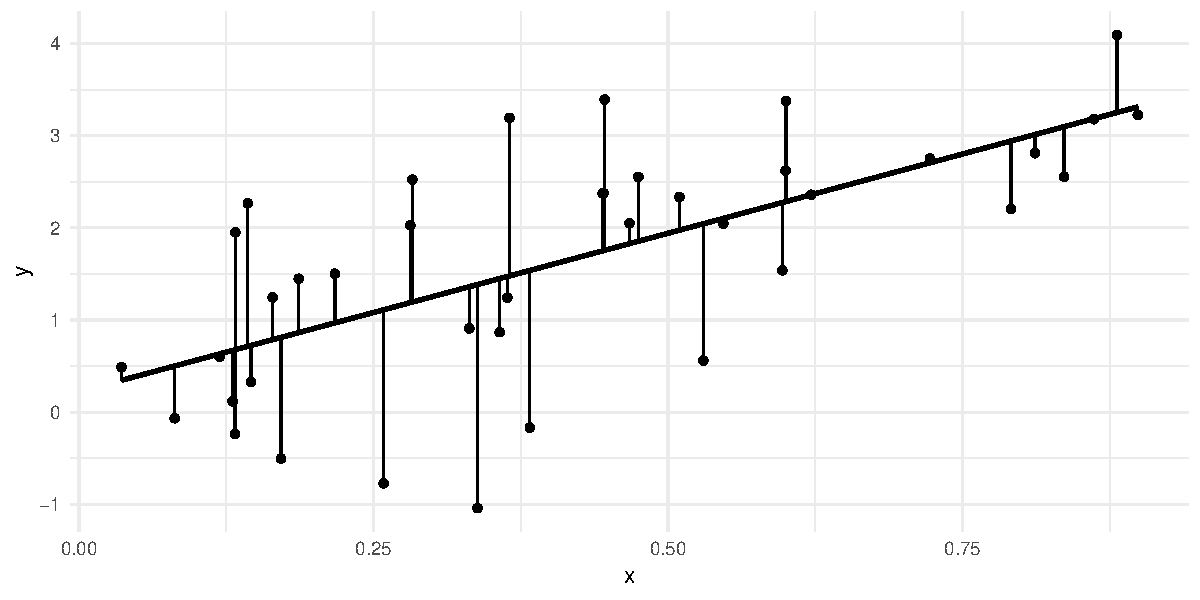
\includegraphics[width=\textwidth]{figures/lm_residuals.pdf}
\caption[Residuals from a simple linear model]{Visualization of residuals
from the linear model $y = \beta_0 + \beta_1 x$.}
\label{lm_residuals}
\end{figure}

%%%%%%%%%%%%%%%%%%%%%%%%%%%%%%%%%%%%%%%%%%%%%%%%%%%%%%%%%%%%%%%%%%%%%%%%%%%%%%
\newpage

\textbf{LAB QUESTIONS}

\vspace*{0pt}

\begin{enumerate}
\item Write Equation~\ref{lloss} as an inner product. Expand and distribute
the terms so that you have a loss function written a linear combination of
matrix products.
\item Convince yourself that the matrix $X^t X$ is equal to its own transpose.
\item Use the gradient rules we had last time to compute the gradient of the
loss function for linear regression.
\item Set the gradient equal to zero. The result is known as the
\textit{normal equations}. Isolate $\beta$ on one side using the matrix inverse.
\item Now, with a known quantity for $\beta$, write down an equation for $\widehat{y}$.
This should take the form:
\begin{align}
\widehat{y} &= H y
\end{align}
For some matrix $H$. The matrix here is called the ``hat'' matrix because it
puts a hat on the quantities of y. Show that $H^2 = HH = H$.
\item Assume that the ``true'' value of $y$ is given by:
\begin{align}
y &= X b + \epsilon
\end{align}
For some vector of random errors $\epsilon$. Plug this into your equation for
$\beta$ and show that $\beta$ can be written as $b$ plus another term that should
be small if the noise terms are small.
\item Show that the residuals ($y - X\beta$) are perpendicular to the fitted
values $\widehat{y}$. That is, show that the dot product between the two is
zero. (Note: you can use the fact that the transpose of $(X^tX)^{-1}$ is equal to itself).
\item Continue by following the notes in the \texttt{class04.Rmd}
\end{enumerate}

\end{document}

